\documentclass[conference]{IEEEtran}
\usepackage{polski}
\usepackage[utf8]{inputenc}
\usepackage{blindtext, graphicx}
\usepackage{float}


\ifCLASSINFOpdf
  % \usepackage[pdftex]{graphicx}
  % declare the path(s) where your graphic files are
  % \graphicspath{{../pdf/}{../jpeg/}}
  % and their extensions so you won't have to specify these with
  % every instance of \includegraphics
  % \DeclareGraphicsExtensions{.pdf,.jpeg,.png}
\else
  % or other class option (dvipsone, dvipdf, if not using dvips). graphicx
  % will default to the driver specified in the system graphics.cfg if no
  % driver is specified.
  % \usepackage[dvips]{graphicx}
  % declare the path(s) where your graphic files are
  % \graphicspath{{../eps/}}
  % and their extensions so you won't have to specify these with
  % every instance of \includegraphics
  % \DeclareGraphicsExtensions{.eps}
\fi


% correct bad hyphenation here
\hyphenation{op-tical net-works semi-conduc-tor}


\begin{document}
%
% paper title
% can use linebreaks \\ within to get better formatting as desired
\title{Obserwacje grup szkolnych w Centrum Nauki Kopernik -- raport}


% author names and affiliations
% use a multiple column layout for up to three different
% affiliations
\author{\IEEEauthorblockN{Ahmed Abdelkarim, Aleksandra Hernik, Ada Wrońska}
\IEEEauthorblockA{Wydział Matematyki i Nauk Informacyjnych\\
Politechnika Warszawska}}

\maketitle


\begin{abstract}
%\boldmath
Celem tego raportu jest przedstawienie wyników analizy danych dotyczących sposobu zwiedzania i charakterystyki dwunastoletnich dzieci w Centrum Nauki Kopernik. Dane składały się z dwóch tabel -- ankiety, która była wypełniana przez dzieci i zawierała informacje na ich temat, które zostały podsumowane jako \textit{kapitał naukowy}, oraz obserwacji dzieci, z takimi informacjami jak czas spędzony przy każdym eksponacie i stopień poświęconej mu uwagi, a także listą innych dzieci biorących udział w interakcji. Przeprowadzoną analizę danych można podzielić na poszukiwanie zależności między pewnymi cechami dzieci (i ich środowiska), znajdowanie prawidłowości w sposobie zwiedzania dzieci, i stworzenie charakterystyki eksponatów.
\end{abstract}
\IEEEpeerreviewmaketitle



\section{Wstęp}
\subsection{Opis danych}
Opisywany projekt polegał na przeanalizowaniu danych z wizyt dwunastoletnich dzieci w Centrum Nauki Kopernik. Dostępne dane znajdowały się w dwóch tabelach:
\begin{itemize}
\item \textit{Ankieta.csv} (237 wierszy), składająca się z: \begin{itemize}
\item ID (numer klasy i ucznia),
\item Informacja, czy uczeń był obserwowany,
\item Płeć,
\item Ukończenie studiów przez rodziców,
\item Praca rodziców,
\item Oceny z matematyki, przyrody i języka polskiego,
\item Wymarzony zawód,
\item Jego pokrewieństwo z nauką,
\item Odpowiedzi na poszczególne pytania z ankiety (poziom kontaktu z nauką).
\end{itemize}
\item \textit{Obserwacje.csv} (15225 wierszy), składająca się z: \begin{itemize}
\item ID ucznia,
\item Nazwa eksponatu,
\item Galeria,
\item Kategoria zdarzenia (przerwa, eksponat i inne),
\item Czas rozpoczęcia, trwania i zakończenia zdarzenia,
\item Osoby towarzyszące w zdarzeniu,
\item Poziom eksploracji eksponatu (patrzenie, dotykanie, używanie lub eksperymentowanie)
\item Informacja o tym, czy dziecko przeczytało opis,
\item Informacja o tym, czy dziecko rozmawiało z animatorem,
\item Uwagi na temat zdarzenia.
\end{itemize}
\end{itemize}
Przed rozpoczęciem analizy dane zostały do niej przygotowane poprzez:
\begin{itemize}
\item Usunięcie brakujących danych (np. nieczytelne pismo jako wymarzona praca),
\item Posortowanie odpowiedzi w ankiecie (factor w~języku R),
\item Poprawienie literówek i usunięcie nadmiarowych spacji w nazwach eksponatów,
\item Usunięcie nieznanych osób towarzyszących.
\end{itemize}
Wstępna analiza danych wykazała, że liczba obserwowanych dzieci, dla których są dane z~ankiety, była bardzo ograniczona (jedynie 79 dzieci). Z~tego powodu konieczne było zrezygnowanie z~niektórych kierunków badań, szczególnie tych, które dotyczyły analizy sposobu zwiedzania przez grupki dzieci -- w~zdecydowanej większości z~nich znajdowały się dzieci, które nie były obserwowane lub nie wypełniały ankiety.
\subsection{Kierunki badań}
Nasza analiza skupiła się na następujących kierunkach badań:
\begin{itemize}
\item Poszukiwanie zależności między różnymi cechami dziecka i jego środowiska,
\item Analiza sposobu zwiedzania przez dzieci, w szczególności obserwacja tworzących się grupek,
\item Analiza eksponatów w Centrum Nauki Kopernik,
\item Wykorzystanie klasteryzacji w celu pogrupowania dzieci i eksponatów.
\end{itemize}

\section{Cechy dzieci i czynniki środowiskowe}

\section{Charakterystyka sposobu zwiedzania przez dzieci}
\subsection{Liczba odwiedzeń eksponatów w zależności od płci}
Na rysunku \ref{odwiedziny_plcie} przedstawiona jest zależność liczby odwiedzonych eksponatów od płci.
\begin{figure}[H]
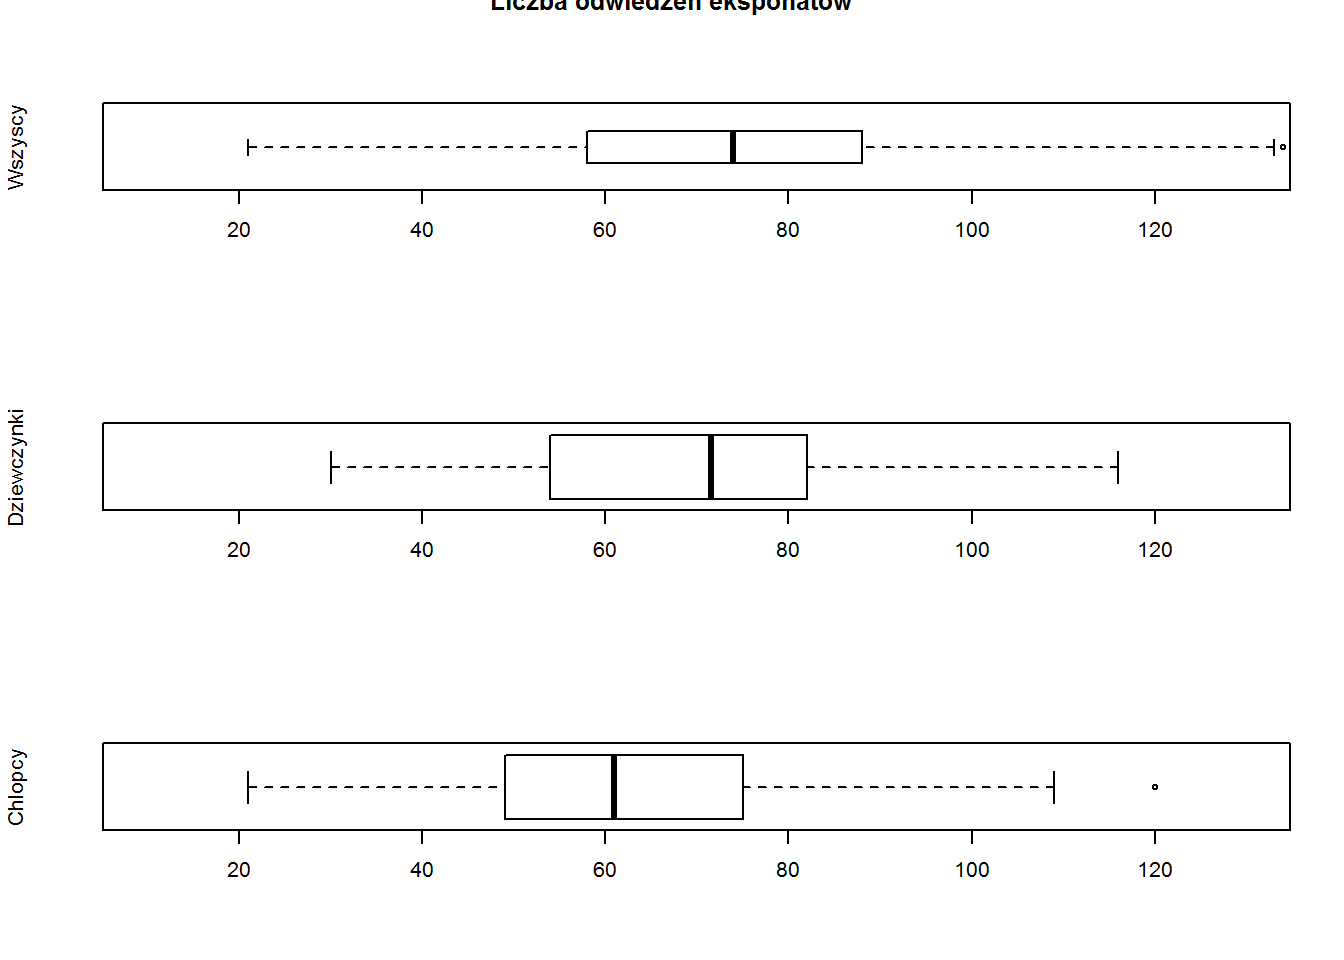
\includegraphics[width=0.48\textwidth]{odwiedziny_plcie.png}
\caption{Liczba odwiedzeń eksponatów w zależności od płci}
\label{odwiedziny_plcie}
\end{figure}
Pierwszy z wykresów przedstawiający odwiedziny wszystkich dzieci zawiera dane o wszystkich dzieciach, a dwa następne jedynie o tych, które wypełniały ankietę -- wskazuje to na istotne braki w danych.

\section{Analiza eksponatów}
\subsection{Popularność galerii}
Rysunek \ref{galerie} przedstawia liczbę odwiedzeń eksponatów w poszczególnych galeriach -- w wersji nieprzetworzonej, a także znormalizowanej ze względu na liczbę eksponatów w galerii.
\begin{figure}[H]
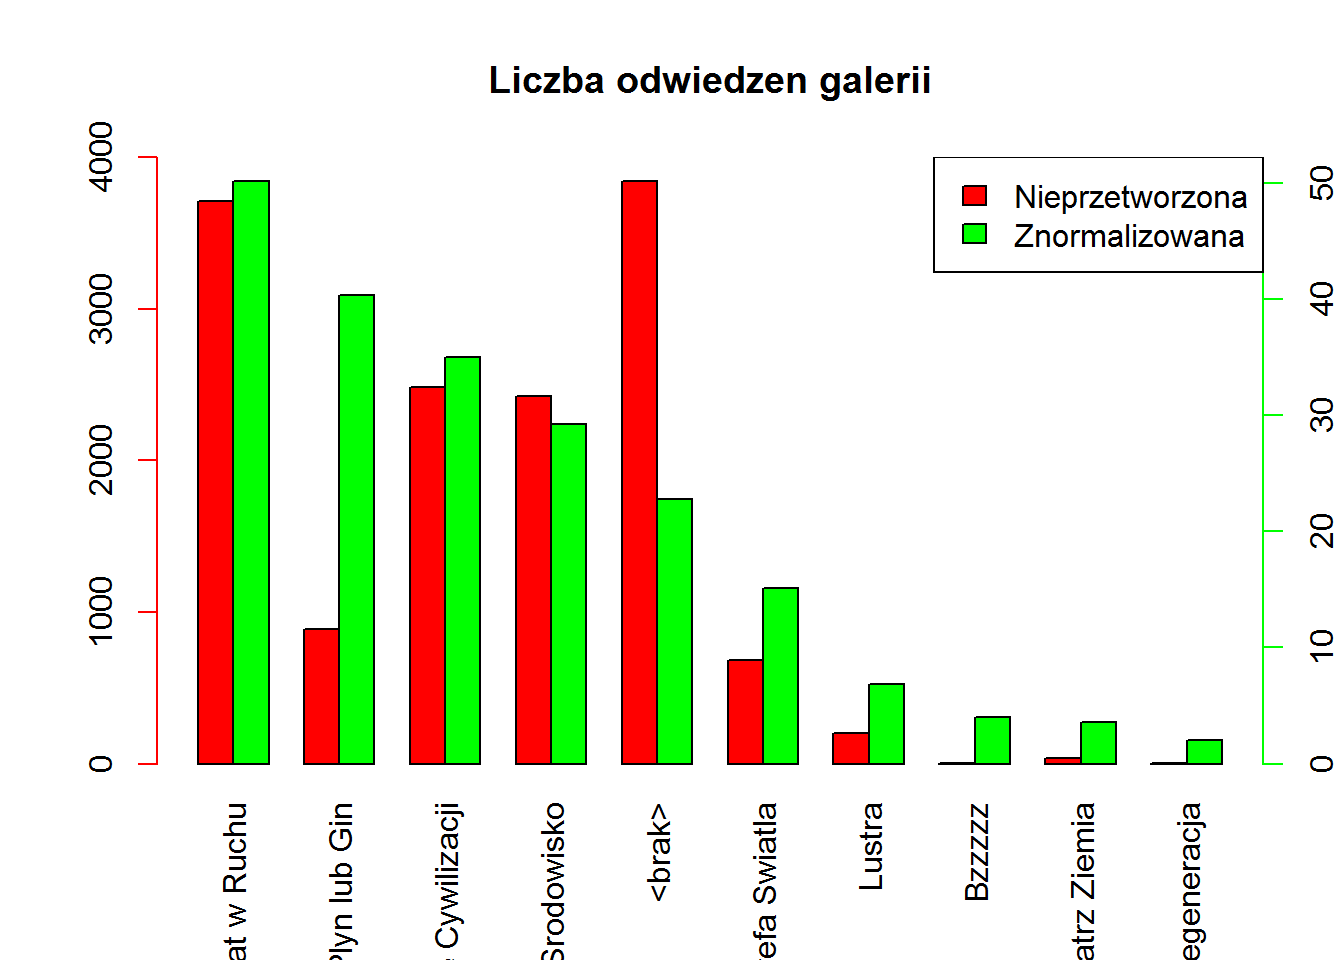
\includegraphics[width=0.48\textwidth]{galerie.png}
\caption{Liczba odwiedzeń poszczególnych galerii}
\label{galerie}
\end{figure}
Normalizacja nie jest w pełni dokładna, ponieważ liczone były jedynie te eksponaty, które zostały odwiedzone co najmniej raz (ze względu na brak kompletnej listy eksponatów) -- anomalie wynikające z tego są szczególnie widoczne w przypadku trzech ostatnich galerii, których liczba odwiedzeń była bardzo niewielka.


\section{Wnioski}








\end{document}


